\documentclass{beamer}

%style
\mode<presentation>{
\usetheme{Warsaw}
\usecolortheme{dolphin}
\setbeamertemplate{navigation symbols}{} % PDF navigationssymbole entfernen
}

%packages
\usepackage[utf8]{inputenc} %deutsche Umlaute
\usepackage[ngerman]{babel} %deutsche Sprache
\usepackage{graphicx} %bilder
\usepackage{booktabs} %for \toprule \midrule \bottomrule in tabellen

%Einstellungen der Präsentation
\title[Präsentations Template]{Präsentations Template}
\author{Stefan Hermes}
\institute[ME]{Home made}
\date{\today}

%Beginn der Präsentation
\begin{document}

%Title
\begin{frame}
\titlepage
\end{frame}

%Inhaltsverzeichnis
\begin{frame}
\frametitle{Inhalt}
\tableofcontents
\end{frame}

%Inhalt
\section{Text}
\subsection{Fließtext}

\begin{frame}
\frametitle{Text}
Ich erzähle was von mir, meiner Arbeit und dem was mein Publikum interessieren könnte.
\end{frame}

\subsection{Gliederung in Bulletpoints}

\begin{frame}
\frametitle{Bulletpoints}
\begin{itemize}
\item enum 1 \pause
\item enum 2
\item enum 3
\end{itemize}
\end{frame}

\subsection{Gliederung in Textblöcken}

\begin{frame}
\frametitle{Textblöcke}

\begin{block}{Textblockname 1}
Text
\end{block}

\pause

\begin{block}{Textblockname 2}
Mehr Text
\end{block}

\begin{block}{Textblockname 3}
Noch mehr Text
\end{block}

\end{frame}

\subsection{Gliederung in Spalten}

\begin{frame}
\frametitle{Mehrere Spalten}
\begin{columns}[c] %c => vertikal zentriert

\column{.4\textwidth} %linke Spalte
\textbf{Linke Spalte}
\begin{enumerate}
\item enum 1
\item enum 2
\item enum 3
\end{enumerate}

\column{.5\textwidth} %rechte Spalte
Hier steht Text der sich auf die linke Spalte bezieht und die einzelnen Punkte erläutert.

\end{columns}
\end{frame}

\section{Tabellen}

\begin{frame}
\frametitle{Tabellen}
\begin{table}
\begin{tabular}{lll}
\toprule
\textbf{Tabellen-} & \textbf{Über-} & \textbf{Schrift} \\
\midrule
Bzgl & Tabellen & gibt \\
es & nichts & Neues \\
\bottomrule
Unter & dem & Strich \\
\end{tabular}
\caption{Beispieltabelle}
\end{table}
\end{frame}

\section{Mathe}

\begin{frame}
\frametitle{Mathematik}
\begin{theorem}[Äquivalenz von Masse zu Welpe]
$K_{itten} = mc^2$
\end{theorem}
\end{frame}

\section{Bilder}

\begin{frame}
\frametitle{Einfügen von Bildern}
Everybody loves kittens \cite{p1}
\begin{figure}
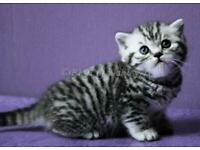
\includegraphics[width=0.7\linewidth]{kitten.jpg}
\end{figure}
\end{frame}

\section{Literatur}

\begin{frame}
\frametitle{Literaturverzeichnis}
\footnotesize{
\begin{thebibliography}{99}
\bibitem[Wikipedia, 2019]{p1}Wikipedia (2019)
\newblock Katezenjunges
\newblock\emph{Wikipedia{,} die freie Enzyklopädie}
\newblock Online; Stand 25. Mai 2019
\end{thebibliography}
}
\end{frame}

\end{document}